\chapter{Approximation Methods}

In theory, the $\varepsilon-$complexity of a continuous function is found using the minimum error over a possibly infinite set of approximation methods. To be computationally efficient, this set of approximation methods needs to be finite and in practice, is restricted to some relatively small set of approximation methods. The initial implementation of the $\varepsilon-$complexity algorithm used piece-wise polynomial interpolation. Our implementation extends the number of methods used to three: basis splines(B-splines) of up to order 5, 
cubic splines and an interpolating subdivision method we refer to as the lifting scheme following Sweldens \cite{sweldens1998}. A fourth method took the minimum error of these three methods at each stage of the $\varepsilon-$complexity algorithm.

The goal of including additional approximation methods was to find whether drawing on a richer set of reconstruction procedures would improve the performance of the $\varepsilon-$complexity coefficients. In this chapter, we gauge the approximation methods in two ways. First, we measure the average approximation error of each method on a range of functions and stochastic processes. We then test the 
ability of the complexity coefficients to discriminate between two sets of simulations with similar parameters. Based on these experiments, increasing the accuracy of the approximation did not lead to better performance in the discrimination task. In fact, the cubic spline method which was less accurate in terms of approximation errors, performed as well or better than the more accurate B-spline method.

A separate concern was the computational efficiency of the approximation methods. Computational efficiency becomes a pressing issue as the size of a data set increases. Although the lifting 
scheme and cubic spline approximation computationally linear 
in their inputs, the cubic spline implementation was the 
fastest method by an order of magnitude. 
 Based on both computational efficiency and classification performance we have used the cubic spline method for computing the complexity coefficients in our \texttt{R} implementation and in the applied work in the following chapters.

\begin{table}[!htbp] \centering 
\begin{tabular}{@{\extracolsep{-6pt}} cccc} 
\\[-1.8ex]\hline 
\hline \\[-1.8ex] 
  Process  & Parameters  & Group 1 & Group 2  \\ \hline 
ARMA        & $p,q $  
            & (-0.1, 0.3), (0.2, 0.1)
            & (0.4, 0.3), (0.1, -0.5)     \\ 
Cauchy      & $\alpha, \beta$   
            & 0.1, 0.5   
            & 0.3, 0.7   \\ 
FARIMA      & $p,d,q$   
            &  (0.1, -0.5),0.3, (0.6, 0.01) 
            & (0.2, -0.4),0.3, (0.4, 0.02)  \\ 
fBm         & $\alpha$   
            & 0.1   
            & 0.3  \\ 
Logistic    & $r$       
            & 3.87   
            & 3.70 \\ 
Rand. Weierstrass &  $\alpha$  & 0.65  & 0.17  \\ 
\hline \\[-1.8ex] 
          \end{tabular} 
  \caption{Simulation parameters for each group.}
  \label{tab:sim-params}
\end{table}


\section{Approximation and Classification Accuracy}

For these experiments, we used six simulations methods comprised of both deterministic and stochastic processes. Two groups of simulations 
were used with two sets of initial parameters for each simulation. The simulations and the 
parameters of each group are listed in Table \ref{tab:sim-params}. 
For each simulation, 30 samples were generated by drawing 
a parameter uniformly from a small window centered on the initial
parameter values. A single sample observation from each simulation group is shown in Figure \ref{fig:jitter-ts}.

% The approximation methods accuracy was compared based on the mean squared error(MSE) of the approximation and secondly the classification accuracy when the complexity coefficients computed by each method were used to classify each simulation. 
For each of the approximation methods we used a 
simple diagnostic plot to check that 
the expected log-log relation of approximation errors $\varepsilon_h$
to the proportion of points used for reconstruction was 
roughly linear. 
Shown in \ref{fig:lift-lm} is an example of log-log linear fit of the approximation errors against the sample fraction for a single function from each simulation type. The lifting method generated these regression plots and the B-spline and cubic spline methods 
resulted in similar regression plots. 

\begin{figure}[!htbp]
  \begin{center}
  % \begin{picture}(60,60)
  % ./figs/coeff-interp-simple-functions1.pdf
  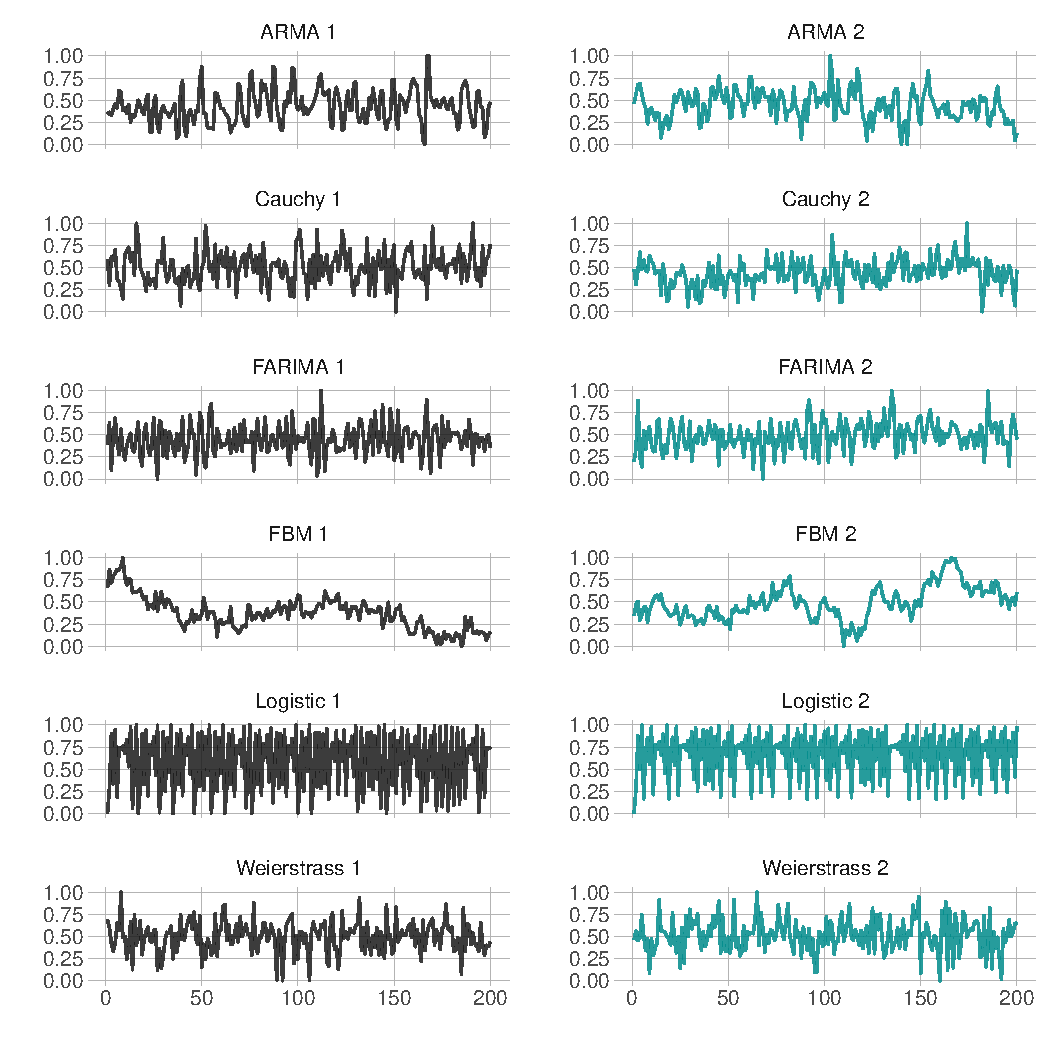
\includegraphics[width = \textwidth, keepaspectratio]{./figs/sim_jitter_plot_jitter_timeseries.pdf}
  % \end{picture}
  \end{center} 
  \caption{Sample functions from each simulation group.  }
   \label{fig:jitter-ts}
\end{figure}


\begin{figure}[!htbp]
  \begin{center}
  % \begin{picture}(60,60)
  % ./figs/coeff-interp-simple-functions1.pdf
  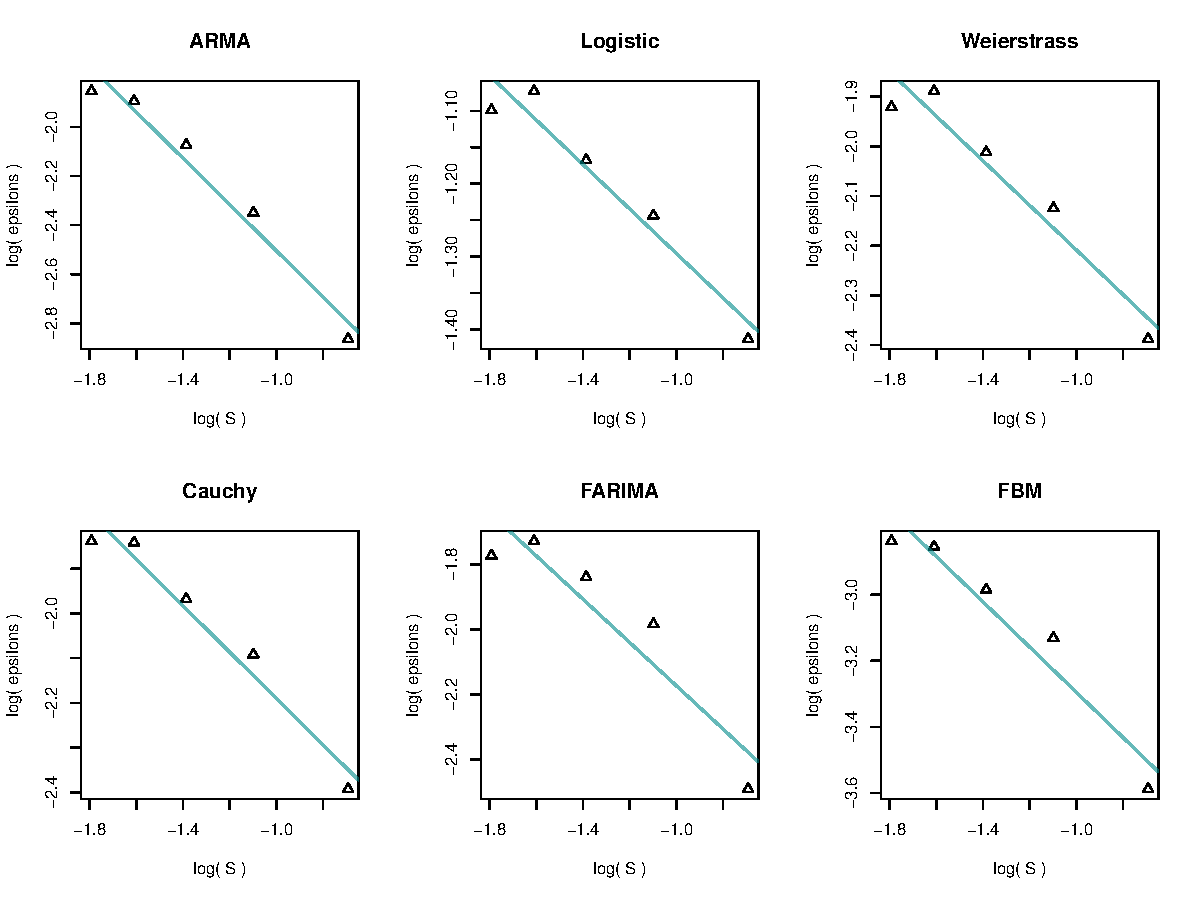
\includegraphics[width = \textwidth, keepaspectratio]{./figs/sim_jitter_plot-sim-fits.pdf}
  % \end{picture}
  \end{center} 
  \caption{Linear regression plots for the lifting scheme.}
  \label{fig:lift-lm}
\end{figure}

\begin{figure}[!htbp]
  \begin{center}
  % \begin{picture}(60,60)
  % ./figs/coeff-interp-simple-functions1.pdf
  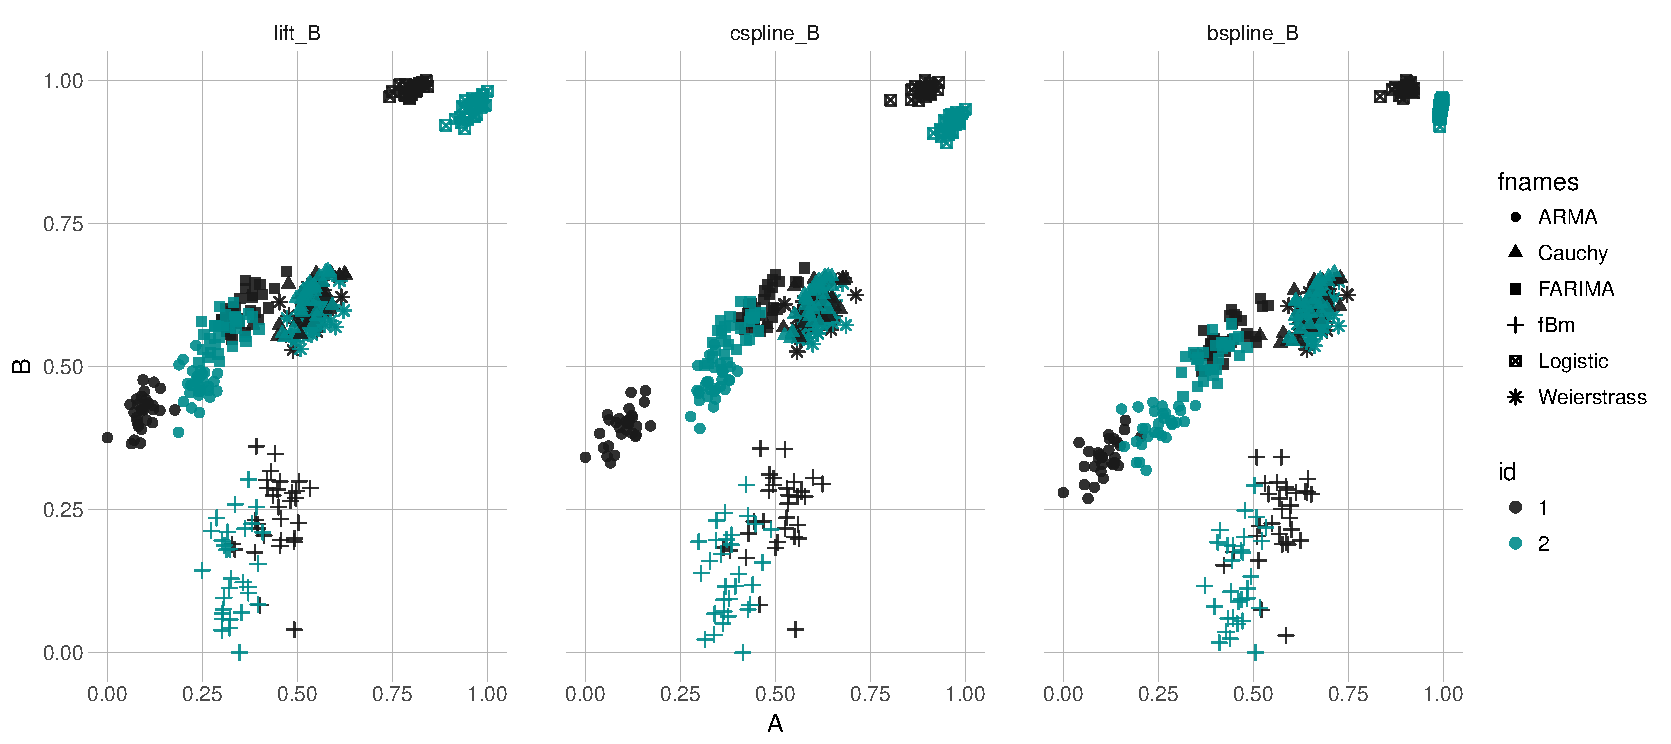
\includegraphics[width = \textwidth, keepaspectratio]{./figs/ecomplex_approx-feature-space.pdf}
  % \end{picture}
  \end{center}
  \caption{The two simulation groups plotted in the 
  complexity coefficient space.}
  \label{fig:feature-space} 
\end{figure}


Figure \ref{fig:feature-space} is a plot of the complexity coefficients generated by each approximation method for the two groups of simulations. Each point represents where an individual function lies in the feature space of the two complexity coefficients $A$ and $B$. The coefficient values have been normalized to the $[0,1]$ interval so the plots show the relative distribution of the functions in the feature space.
Although we quantify the ability of the approximation methods to 
separate each group, the scatter plots show that the methods 
place each simulation type at similar coordinates in the 
complexity coefficient space. The scatter plots also show 
that some methods separated the particular processes better. 
For example, the cubic spline method separates the two groups 
generated by ARMA(2,2) processes.

\begin{figure}[!htbp]
  \begin{center}
  % \begin{picture}(60,60)
  % ./figs/coeff-interp-simple-functions1.pdf
  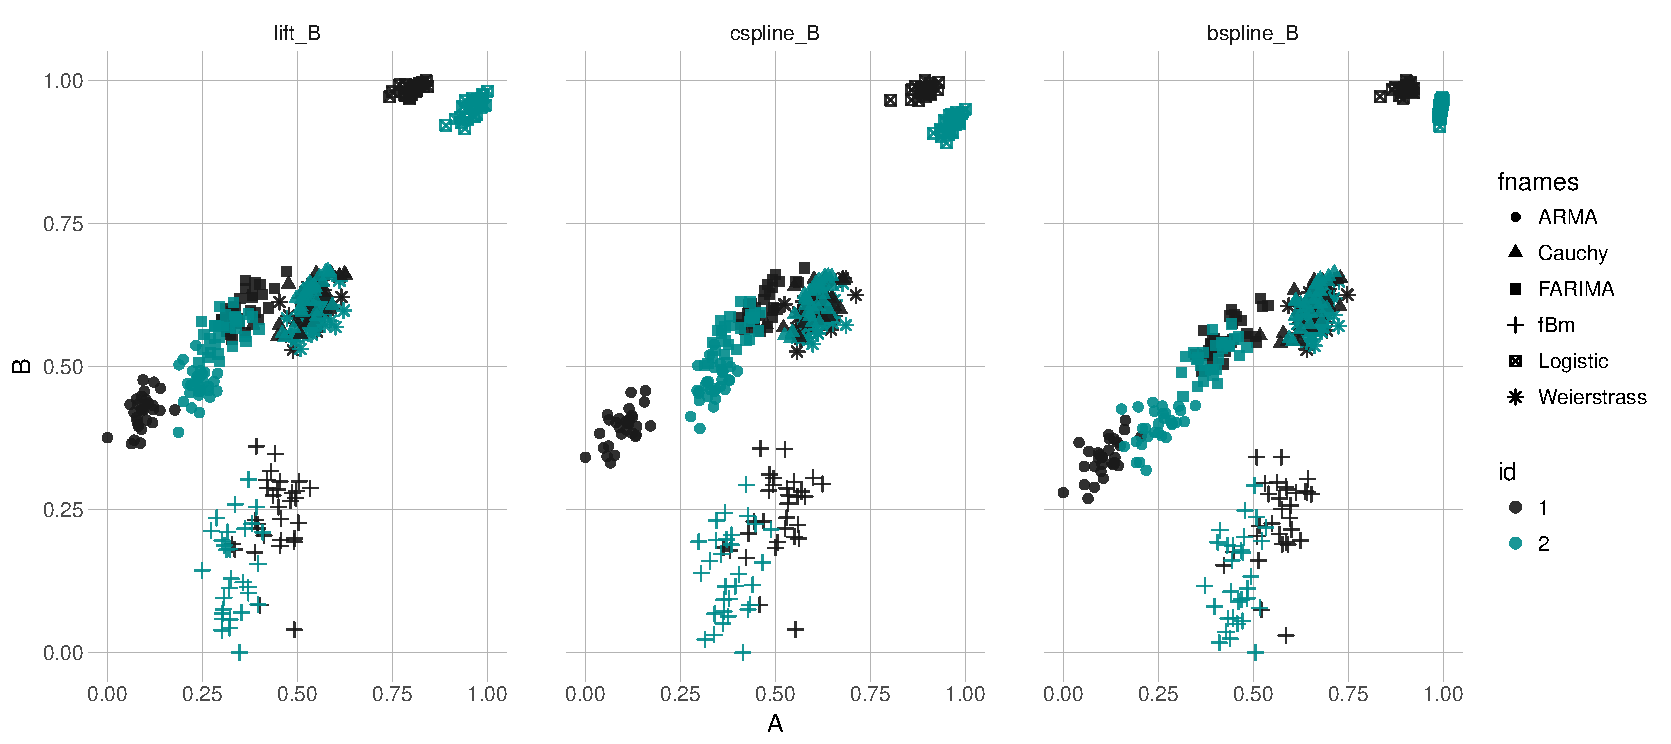
\includegraphics[width = \textwidth, keepaspectratio]{./figs/ecomplex_approx-feature-space.pdf}
  % \end{picture}
  \end{center}
  \caption{Functions from the two simulation groups plotted in the 
  complexity coefficient space.}
  \label{fig:feature-space} 
\end{figure}

The scatter plot of the simulations also provides some information 
about the angle at which the simulations are separable.
 % In the following chapter, we compare how the complexity coefficients and fractal dimension vary with the parameters several functions. Based on those tests it is unclear whether the intercept coefficient $A$ adds contributes information that can be used in discriminating two functions that are not found in slope coefficient $B$.
 % and the variogram estimator of fractal dimension were reflected changes in the parameters controlling the H\"older class of the function. 
 % Except in the case of the random phase Weierstrass function, the intercept coefficient $A$ seemed to follow a similar pattern as the slope coefficient. 
 Figure \ref{fig:feature-space} shows that for the function types that are readily separable --- fBm and the ARMA and logistic simulations ---  both the slope and intercept coefficient appear to be useful in separating the two sets of simulations. For example, both the fBm and ARMA simulations are well separated along the $A$-axis. On the other hand, the realizations of the logistic map in the upper right hand corner appears separable on the diagonal meaning both complexity coefficients contributed to differentiating the two simulation groups.

Using the two sets of simulations described above, with 30 samples taken from each parameter group, the sum of the errors of 
each methods was calculated. 
Table \ref{tab:epsilons-all} show the mean approximation error 
over the 30 samples. The approximation error was calculated by 
taking a simple sum of errors at each down sampling level $h$: 
\[
  \varepsilon_{\mathcal{F}} = \sum_{h} \varepsilon_{h, \mathcal{F}}
\]
The B-spline method had the lowest MSE for all processes.
Since the B-spline method produced the minimum 
error for each function, the combined method 
simply reflects that of the B-spline approximation
\ref{tab:error-mse}.
The lifting method produced a slightly lower mean error but 
the cubic and lifting errors are very similar for each
simulation. 

\begin{table}[!htbp] \centering 
\begin{tabular}{@{\extracolsep{1pt}} ccccccc} 
\\[-1.8ex]\hline 
\hline \\[-1.8ex] 
  Function & Lift & Cspline & Bspline & Combined \\ \hline 
ARMA       & 0.10  & 0.11    & 0.07 & 0.07 \\ 
Cauchy       & 0.09  & 0.10  & 0.06 & 0.06 \\ 
FARIMA       & 0.13  & 0.14  & 0.08 & 0.08 \\ 
fBm          & 0.03  & 0.04  & 0.02 & 0.02 \\ 
Logistic     & 0.30  & 0.32  & 0.20 & 0.20 \\ 
Weierstrass  & 0.14  & 0.15  & 0.09 & 0.09 \\ 
\hline \\[-1.8ex] 
          \end{tabular} 
  \caption{Mean total approximation error for 30 samples of each simulation. 
             }
  \label{tab:epsilons-all}
\end{table}


\begin{table}[!htbp] \centering 
\begin{tabular}{@{\extracolsep{1pt}} ccccccc} 
\\[-1.8ex]\hline 
\hline \\[-1.8ex] 
Function    &  Lift & Cspline & Bpsline  & Combined 
                                       \\ \hline
ARMA        & 0.03 &   0.00 &   0.07 &   0.07  \\ 
Cauchy      & 0.65 &   0.53 &   0.52  &    0.53  \\ 
FARIMA      & 0.32 &   0.30 &   0.32  &    0.33 \\ 
fBm         & 0.20  &   0.22  & 0.20 &  0.22  \\ 
Logistic    & 0.00 &   0.00 &   0.00  &    0.02  \\ 
Weierstrass & 0.50 &   0.43 &   0.45  &    0.45  \\
\hline \\[-1.8ex] 
          \end{tabular} 
  \caption{Classification errors using complexity coefficients  
  $A$ and $B$ for each approximation method using a random 
  forest classifier.}
  \label{tab:error-all}
\end{table}

The set of complexity coefficients as computed by each 
approximation method were then used to classify the 30 samples from each simulations. The classifier was a random forest with 
500 trees with 3 features used to determine branches. The overall out-of-bag classification error is reported in \ref{tab:error-all}. The cubic 
spline method performed equally well or better
on 4 of the 6 methods, but the results of all methods are 
similar.

% Finally we tested whether the classification error varied with the loss function used to compute approximation error. Again, accuracy computed as the out-of-bag classification accuracy of a random forest classifier. Both the mean squared error, mean absolute error(MAE) loss function performed similarly with MAE performing slightly better. 

% \begin{table}[!htbp] \centering 
% \begin{tabular}{@{\extracolsep{1pt}} ccccccc} 
% \\[-1.8ex]\hline 
% \hline \\[-1.8ex] 
% Function     &   MAE  &  MSE   & Max \\
% ARMA         &   0.00  &  0.03  & 0.33 \\ 
% Cauchy       &   0.52  &  0.66  & 0.47 \\ 
% FARIMA       &   0.18  &  0.22  & 0.39 \\ 
% fBm          &   0.13  &  0.16  & 0.33 \\ 
% Logistic     &   0.01  &  0.00  & 0.18 \\ 
% Weierstrass  &   0.44  &  0.53  & 0.51 \\
% \hline \\[-1.8ex] 
%           \end{tabular}  
%   \caption{Classification error using a random forest clasysifier 
%            and three different loss functions.}
%   \label{tab:error-mse}
% \end{table}

\section{Computational Complexity}

 Classification performance was not affected by the slightly lower approximation accuracy of the lifting and cubic spline methods. However, both the cubic spline and lifting approximation methods are computationally more efficient than the B-spline method. Both methods are linear in the number of inputs and both are linear or constant in terms of their space complexity, that is, 
the amount of memory needed to store intermediate computations is a linear or constant function of the size of the inputs. 

The execution time of each approximation method estimated
using the system time taken to complete approximations on 
inputs of size $10^7$ to $10^{13}$. 
The average computational time for
each input size on log-scale is shown in Figure \ref{fig:benchmark}.
For our implementation, 
the B-spline method expands the number of knots linearly with 
the inputs. This leads to the B-spline method becoming 
infeasible for even moderately large inputs. 
Although the cubic spline and lifting method are computationally 
linear, the lifting scheme was implemented entirely in the \texttt{R}
language. The cubic spline method is called from \texttt{R} but 
most calculations are written in the computationally efficient \texttt{C} language. Although it is not clear in Figure 
\ref{fig:benchmark}, the cubic spline method was an order of magnitude faster than the lifting scheme. 

\begin{figure}[!htbp]
  \begin{center}
  % \begin{picture}(60,60)
  % ./figs/coeff-interp-simple-functions1.pdf
  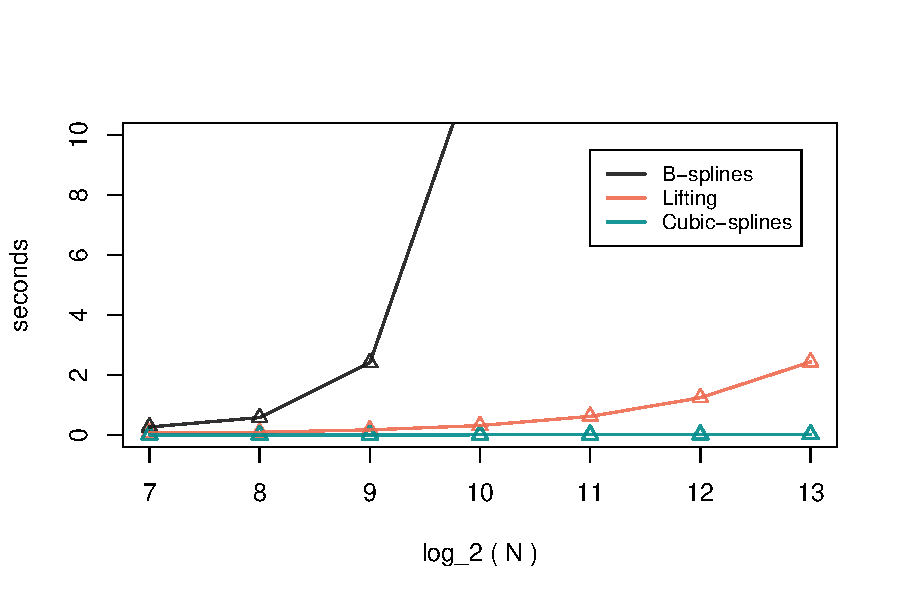
\includegraphics[width = \textwidth, keepaspectratio]{./figs/benchmark-benchmark.pdf}
  % \end{picture} 
  \end{center}
  \caption{Computational time as a function of the 
  size of the input.}
  \label{fig:benchmark} 
\end{figure}

% Since both complexity coefficients were useful 
% in discriminating between functions drawn from similar sets of parameters, we also used both coefficients to 

Our primary goal of the preceding test was to determine 
if enlarging the set of approximations would lead to improved 
performance of the complexity coefficients. We assumed 
that the enlarged set would allow for improved approximation error 
and a better estimation of the complexity coefficients. 
Here we measured 
performance by the ability of the complexity coefficients to 
discriminate between closely related simulations. Lower 
approximation errors did not correspond to better classification
accuracy, however. The cubic spline method was the most computationally efficient and performed as well or better on the classification test as the other methods. Based on these results,
the cubic spline approximation was used for the applied work in 
Chapters 4 and 5.






